\documentclass{sigchi-ext}
% Please be sure that you have the dependencies (i.e., additional
% LaTeX packages) to compile this example.
\usepackage[T1]{fontenc}
\usepackage{textcomp}
\usepackage[scaled=.92]{helvet} % for proper fonts
\usepackage{graphicx} % for EPS use the graphics package instead
\usepackage{balance}  % for useful for balancing the last columns
\usepackage{booktabs} % for pretty table rules
\usepackage{ccicons}  % for Creative Commons citation icons
\usepackage{ragged2e} % for tighter hyphenation

% Some optional stuff you might like/need.
% \usepackage{marginnote} 
% \usepackage[shortlabels]{enumitem}
% \usepackage{paralist}
% \usepackage[utf8]{inputenc} % for a UTF8 editor only

%% EXAMPLE BEGIN -- HOW TO OVERRIDE THE DEFAULT COPYRIGHT STRIP --
% \copyrightinfo{Permission to make digital or hard copies of all or
% part of this work for personal or classroom use is granted without
% fee provided that copies are not made or distributed for profit or
% commercial advantage and that copies bear this notice and the full
% citation on the first page. Copyrights for components of this work
% owned by others than ACM must be honored. Abstracting with credit is
% permitted. To copy otherwise, or republish, to post on servers or to
% redistribute to lists, requires prior specific permission and/or a
% fee. Request permissions from permissions@acm.org.\\
% {\emph{CHI'14}}, April 26--May 1, 2014, Toronto, Canada. \\
% Copyright \copyright~2014 ACM ISBN/14/04...\$15.00. \\
% DOI string from ACM form confirmation}
%% EXAMPLE END

% Paper metadata (use plain text, for PDF inclusion and later
% re-using, if desired).  Use \emtpyauthor when submitting for review
% so you remain anonymous.
\def\plaintitle {Title} \def\plainauthor{First Author, Second Author, Third Author, Fourth Author}
\def\emptyauthor{}
\def\plainkeywords{Mediated Reality; Augmented Reality; Wearable Computing;
Sequential Wave Imprinting Machine; WearTech, Lock-In amplifier;
HARCAD/HARCAM; Haptic Augmented Reality CAD/CAM}
\def\plaingeneralterms{Augmented Reality, Visualization}

\title{Phenomenologically Augmented Reality With New Wearable LED Sequential Wave Imprinting Machines}

\numberofauthors{4}
% Notice how author names are alternately typesetted to appear ordered
% in 2-column format; i.e., the first 4 autors on the first column and
% the other 4 auhors on the second column. Actually, it's up to you to
% strictly adhere to this author notation.
\author{%
  \alignauthor{%
    \textbf{Pete Scourboutakos}\\
    \affaddr{University of Toronto} \\
    \affaddr{Toronto, ON M5S 3G4, Canada} \\
    \email{pete@eyetap.org} }\alignauthor{%
    \textbf{Max Hao Lu}\\
    \affaddr{University of Toronto} \\
    \affaddr{Toronto, ON M5S 3G4, Canada} \\
    \email{max@eyetap.org} } \vfil \alignauthor{%
    \textbf{Sarang Nerker}\\
    \affaddr{University of Toronto} \\
    \affaddr{Toronto, ON M5S 3G4, Canada} \\
    \email{sarang@eyetap.org} }\alignauthor{%
    \textbf{Steve Mann}\\
    \affaddr{University of Toronto / WearTech\texttrademark Foundation} \\
    \affaddr{Toronto, ON M5S 3G4, Canada} \\
    \email{mann@eyetap.org} } }

% Make sure hyperref comes last of your loaded packages, to give it a
% fighting chance of not being over-written, since its job is to
% redefine many LaTeX commands.
\definecolor{linkColor}{RGB}{6,125,233}
\hypersetup{%
  pdftitle={\plaintitle},
%  pdfauthor={\plainauthor},
  pdfauthor={\emptyauthor},
  pdfkeywords={\plainkeywords},
  bookmarksnumbered,
  pdfstartview={FitH},
  colorlinks,
  citecolor=black,
  filecolor=black,
  linkcolor=black,
  urlcolor=linkColor,
  breaklinks=true,
}

% \reversemarginpar%

\begin{document}

%% For the camera ready, use the commands provided by the ACM in the Permission Release Form.
%\CopyrightYear{2007}
%\setcopyright{rightsretained}
%\conferenceinfo{WOODSTOCK}{'97 El Paso, Texas USA}
%\isbn{0-12345-67-8/90/01}
%\doi{http://dx.doi.org/10.1145/2858036.2858119}
%% Then override the default copyright message with the \acmcopyright command.
%\copyrightinfo{\acmcopyright}

\maketitle

% Uncomment to disable hyphenation (not recommended)
% https://twitter.com/anjirokhan/status/546046683331973120
\RaggedRight{} 

% Do not change the page size or page settings.
\begin{abstract}
%  UPDATED---\today. This sample paper describes the formatting
%  requirements for SIGCHI Extended Abstract Format, and this sample
%  file offers recommendations on writing for the worldwide SIGCHI
%  readership. Please review this document even if you have submitted
%  to SIGCHI conferences before, as some format details have changed
%  relative to previous years. Abstracts should be about 150
%  words. Required.
   The Sequential Wave Imprinting Machine (SWIM),
   invented by Steve 
   Mann in the 1970s, offers naked-eye augmented reality overlays
   with perfect alignment,
   through a Persistence of Exposure (PoE) of human vision,
   or photographic/videographic media.
    
   This paper proposes a 
   new SWIM design with only 2 transistor elements per picture elment,
   therefore making SWIM more wearable, miniature, and affordable.
   We present a SWIM for being worn on one finger, as a ring, to overlay
   a phenomenologically augmented reality for metaveillance
   (sensing sensors and sensing their capacity to sense)
   and HARCAD (Haptic Augmented Reality Computer Aided Design/Manufacture).
\end{abstract}

\keywords{\plainkeywords}

\category{H.5.m}{Information interfaces and presentation (e.g.,
  HCI)}{Miscellaneous}
%\category{See}{\url{http://acm.org/about/class/1998/}}{for
%  full list of ACM classifiers. This section is required.}

\section{Introduction}
Augmediated reality is an experience where by the means of a system of
technology, people are able to seamlessly modify (mediate) their
perception of reality, while it is also being augmented.

Mediated reality systems may be organized into three types:
\begin{enumerate}
\vspace{-.15in}
 %\setlength\itemsep{-1em}
 \item dB\textgreater  0: Systems of augmentation, which involve amplification / enhancement / addition of information, such as the system presented here. These systems are augmented reality.
 \item dB\textless  0: Those of diminishment which involve
attenuation / subtraction of vision, like dark glass or even
HDR vision glass for welding~\cite{mannHDR}.
These systems are useful where diminished reality is desired.
 \item Those which are dynamic and can do both, as needed.
%\vspace{-.5in}
\end{enumerate}
Many augmediated reality systems are of the third type, designed as a
generalized platform with the intention of supporting a variety of
applications~\cite{arsurvey}. These
%, which is in line with the way most personal computers (including
%smartphones) are thought of as being interacted with
systems consist of input and output devices,
respectively, with computer processing in
between~\cite{mann2012realtime, mann1998wearable, mann1998humanistic,
mann2001wearable}.

%Thanks to ongoing advancements in miniturization and wearable computer
%technology, there is large scale interest and commercial development ongoing in
%these areas~\cite{mann1998wearable}. The challenge with a system of this
%complexity is for it to embody the principles of humanistic
%intelligence~\cite{mann1998humanistic}
%which are key to a system which will provide a
%seamless and convincing experience which can advance technology for
%humanity~\cite{mann2001wearable}.

The augmediated reality system in this paper is strictly additive (type 1). It
is also purpose built for the specific application of the visualization of
radio waves, in the same fashion as early augmediated reality experiments
carried out by Steve Mann in the 1970s~\cite{mann2015phenomenal}
(See Fig.~\ref{fig:swim74}).
\begin{marginfigure}[-25pc]
  \begin{minipage}{\marginparwidth}
 \includegraphics[width=\textwidth]{SteveMann_SequentialWaveImprintingMachine_AR_wand_6502-44_nan_crop.png}
 \includegraphics[width=.8\textwidth]{SittingWaveTwoCycles4crop.jpg}
 \includegraphics[width=.8\textwidth]{hello2cropcrop.jpg}
    \centering
    \caption{
             World's first wearable augmented reality computer system:
             Sequential Wave Imprinting Machine waved back-and-forth
             to display
             radio waves, sound waves, text, graphics, etc.,
             overlaid on reality by persistence-of-exposure,
             so hundreds of people could see the
             overlay without the need to wear special eyeglasses.
            }
    \label{fig:swim74}
  \end{minipage}
\end{marginfigure}
Recently, with the availability of high efficiency and small SMD LEDs, the SWIM
no longer relies on incandescent light bulbs and has thus become more
practical.

This paper presents two new incarnations of SWIM. The first is based on
surface mount version of the
LM3914 (Fig.~\ref{fig:schematic3914})
and provides high resolution (10pixels/cm) at a modest
board size. The second is a novel circuit which is used to make a small
wearable SWIM which is unprecedented in miniaturization,
making these experiments in augmediated reality ever more practical
as a wearable computer, and also making it possible, if desired, to
further miniaturize the apparatus into a single die chip for use in eyeglasses
or contact lens displays [Mann 1999, CA2280022],
with just two transistor elements per pixel
(Fig.~\ref{fig:schematictransistors}).

%LED technology has existed since the 1970s (60s?) but until the last decade remained only practical for low light applications of indication, due to a severe limitation in light output compared to other sources of light such as incandescants, or fluourescents. Recent advances in semiconductor device design for LEDs has made LEDs practical for applications of lighting and display beyond simple indication, as made apparant by the availablilty of LED televisions in (2009/2012 Sony).[wikipedia, how do we cite something like this? cite a product]\\

Head mounted displays~\cite{mann1997wearable}, have been used extensively as
the output device of choice for augmediated reality
systems~\cite{caudell1992augmented}.
This is natural because they are usually already
designed to work as computer displays. These types of devices are well suited
to personal augmediated reality experiences, but do not work as easily for
activities where multiple people or groups of people are involved and wish to
partake in the same experience. For everyone to participate, everyone must wear
their own pair of glasses, and high level software/networking systems are
required to render the experience for everyone. This creates bottleneck points
and opens up opportunities for delays and other issues which can strip the
system of its humanistic intelligence, making the experience anything from less
convincing to illness-inducing to painful~\cite{drascic1996perceptual}.
\begin{figure}
 \centering
 \includegraphics[scale = 0.274, angle = 270]{3914schem.pdf}
 \caption{Schematic of modular LM3914 SWIM device.}
 \label{fig:schematic3914}
\end{figure}
SWIM eliminates the complexity imposed by the need for a general
purpose system, and instead focuses as a single-purpose-built augmediated
reality system which makes visible normally invisible radio waves. In order to
achieve this effect, the SWIM is simply driven with the doppler return output
of any low power X band microwave radar set.

SWIM works similarly to an oscilloscope with no timebase generator, by painting out a sensed/measured wave in light so that it is made visible. Instead of the effect of the oscilloscope phosphor we have the phenomenon of persistance of exposure~\cite{mann2015phenomenal}. An oscilloscope works in real-time but virtual-space, on its own 2D display, like most AR systems, while the SWIM uses a 1D display to produce an image like a 2D holograph, which is registered in real-time as well as in real-space, as the user sweeps the SWIM device itself through the waves in space. 
Last and perhaps most importantly, the augmediated reality experience SWIM
creates is easily shared among a group of people, all of whom may bear witness
with the naked eye, as shown in Fig.~\ref{fig:stuffie}.
\begin{figure}
 \centering
 \includegraphics[width=.5\textwidth]{schematic.pdf}
 \caption{Schematic of  novel discrete transistor LED SWIM device.}
 \label{fig:schematictransistors}
\end{figure}

\begin{marginfigure}[-23pc]
  \begin{minipage}{\marginparwidth}
 \includegraphics[width=\textwidth]{sarangs.jpg}\\
 \includegraphics[width=\textwidth]{microswims.jpg}\\
 \includegraphics[width=\textwidth]{SDC11632s.jpg}\\
 \includegraphics[width=\textwidth]{SWIMs.jpg}
    \centering
    \caption{Wearable augmented reality without special eyeglasses.
             Wristworn and finger-worn.
             The ``SWIM ring'' is compact, wearable, lightweight,
             and easy to use.
             Waving the ring back and forth makes metaveillance waves
             visible.
            }
    \label{fig:stuffie}
  \end{minipage}
\end{marginfigure}

\section{Recent Advances in SWIM}
Recently SWIM (and augmented reality in general)
has attracted considerable interest, and many are being built.
The simplest to implement were digital, with a microcontroller
driving cascaded serially programmable WS2812 RGB "neopixels", which can
conveniently be purchased in a strip, but pixels are large (greater than 0.5cm)
and they suffer from a limited refresh rate.  SWIMs of the
1980s and '90s were built around the
LM3914 cascadable 10 segment dot/bar graph display driver IC, which produces
excellent results with a high degree of accuracy, tested up to 200
cascaded ICs for HD pixel counts (2000 pixels)
and large scale size.  This modular design used
is seen in Fig.2.  The LM3914 was measured to have a bandwidth around
1.6Mhz,
which translates to a very high "refresh rate" and the simple analog system
controlling it approaches linear time invariancy, eliminating the possibility
of any lag.  Thus the system always responds instantly and the experience is
seamless and convincing: humanistic integrity is maintained.
LM3914 ICs were
used to make a wristworn "microswim" pictured in Fig.4, which is a 60 pixel
SWIM, utilizing 0603 size SMD LEDs, which fits on a 6cm square PCB
(its image also shown in the same figure).
A novel discrete transistor circuit
has been devised, pictured in Fig.3, which makes a low pixel count SWIM smaller
and cheaper than is possible with the LM3914. Pictured also in Fig. 4
is an 8 pixel
discrete SWIM (fits on a 1.25cm by 1.9cm PCB small enough to be worn a ring)
together with its output image.
%
%\section{Visualization of Waves with the Sequential Wave Imprinting Machine}
%One important application of augmediated reality is for making visible the invisible world. It is known that invisible radio %waves are everywhere, permeating all space around us, and thus if these waves are made visible by some means, more may be learned of the world that surrounds us and the way it works. 
%This is the ethos which led Steve Mann to develop the Sequential Wave Imprinting Machine as a teenager in the 1970s. The device was a general purpose analog or digitally controllable linear display of lightbulbs, with which he was able to visually witness (visualize) radio waves in real-time as well as real-space. The device is designed to operated in a simple manner, it is waved about by the user, and as it moves through space, it paints out in light [cite lightpainting? abakographic user interfaces] the radio waves produced by an accompanying radar set.

%When in a dark place or where the ambient light can be controlled to a low level, the system works by the phenomenon of persistance of exposure[cite mann] and makes waves able to be observed with the naked eye by the user as well as onlookers. 

\section{Tactile SWIM for Haptic Augmented Reality CAD/M}
Some of the early embodiments of SWIM began as electromechanical devices,
which naturally lent themselves to being grasped, held, touched, etc..
One of Mann's early experiments was to use an X-Y plotter to visualize
(and feel) radio waves, sound waves, and the like
(Fig.~\ref{fig:plotter}).
\begin{figure}
  \includegraphics[width=\linewidth]{tswim_XYplotter_cp_lowres.jpg}
  \caption{Mann's early haptic radio wave experiment using X-Y plotter
           to touch, feel, and grasp hold of radio waves in perfect alignment
           with reality, due to simple physical phase-coherent detection.
 (visuals from single light bulb + haptics).
%           The X-axis servo is disabled so the user can slide it freely
%           left-to-right while the Y-axis is driven by the output of
%           a lock-in amplifier connected to a stationary reference
%           antenna and a moving signal antenna.
          }
  \label{fig:plotter}
\end{figure}
This gives way to haptics for collaboratively creating physical objects:
HARCAD
(Fig.~\ref{fig:tswims}),
a system to
explore ``Cyborg Craft'', a new kind of undigital craft: being undigital
with digital computers.
%One such embodiment is the T-SWIM
%(Figs~\ref{fig:plotter} and~\ref{fig:tswims}),
%as a haptic augmented reality interaction devices and systems.
In this system, one or more users can grasp and touch and feel virtual
objects in cyborgspace, and share the resulting haptic augmented reality
experience, as a way of designing and making things like cars,
buildings, furniture, etc., through a collaborative design and
realization process.

\begin{marginfigure}[-20pc]
  \begin{minipage}{\marginparwidth}
  \includegraphics[width=\linewidth]{threefundamentals_and_me_dccq.jpg}
  \includegraphics[width=\linewidth]{wave87_and_me90_dccq.jpg}
  \includegraphics[width=\linewidth]{WaveTableFusion360.png}
  \includegraphics[width=\linewidth]{wavetable_20161129_214045cq.jpg}
    \centering
    \caption{
           {\bf Furniture design with Haptic Augmented Reality
                CAD/CAM}.
           A shape synthesizer generates shape information which is
           visualized in alignment with haptic sensation, so shapes can
           be seen and felt in perfect alignment.
           A 3D (3-dimensional) wireless position sensor comprises
           transducers with phase-coherent detection.
Ultimately we bypass CAD altogether to directly and collaboratively
interact with the manufacturing process.  That's what we call
``undigital cyborg craft''.
%           The synthesizer is connected to a fixed transducer (loudspeaker),
%           and the reference input of a NARLIA (Natural Augmented Reality
%           Lock-In Amplifier).  A moving transducer (microphone) on a
%           Haptic Augmented Reality CAD (HARCAD) wand is connected to the
%           signal input of the NARLIA.
%           An output from the NARLIA is connected to a T-SWIM, here, 600
%           LEDs and a vibrotactile actuator, both part of the HARCAD wand.
%           As the user moves the wand back-and-forth, a multisensory
%           experience results in which the user can see, feel, and
%           hear the virtual shapes (e.g. waves and their harmonics).
%           Arbitrary shapes can be generated by Fourier synthesis,
%           and these shapes can be touched, felt, and manipulated.
            }
    \label{fig:wavetable}
  \end{minipage}
\end{marginfigure}

\begin{figure}
  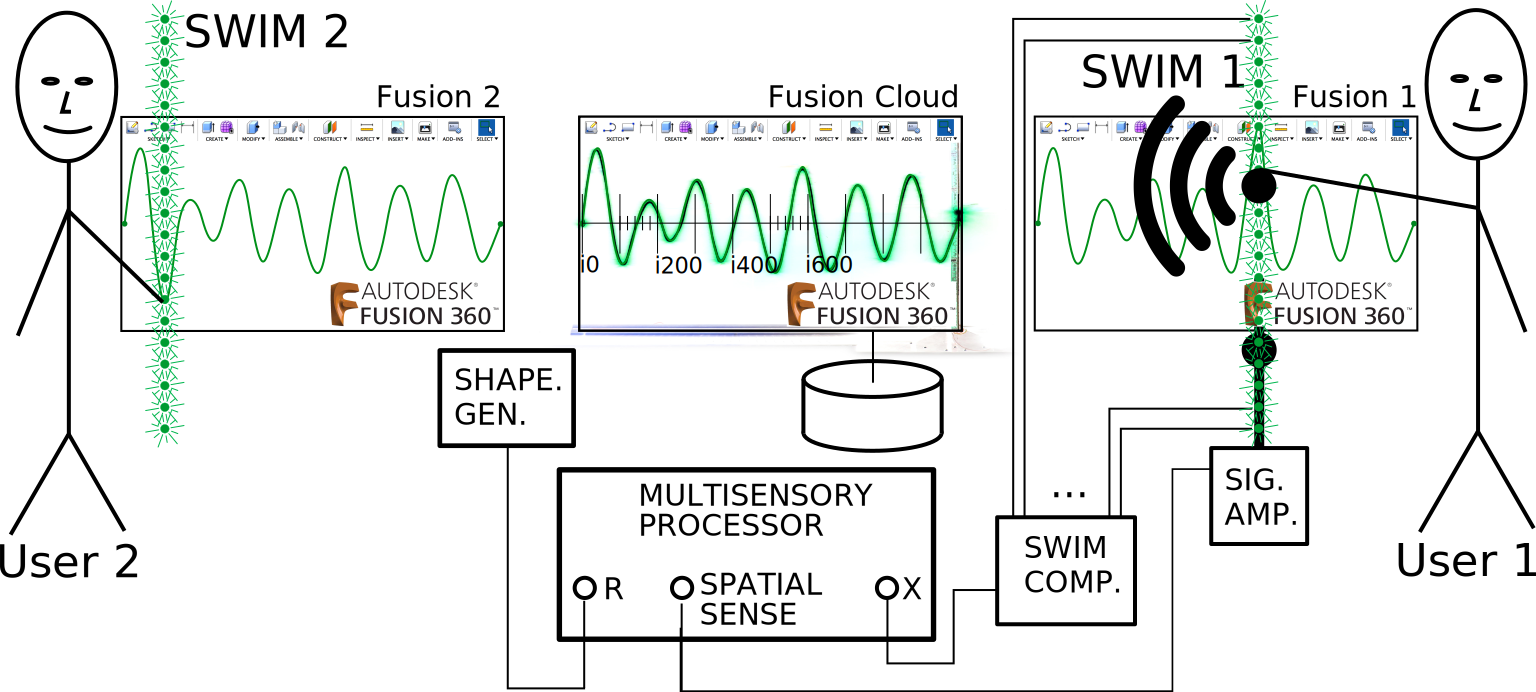
\includegraphics[width=\linewidth]{fig2tei.pdf}
  \caption{
           HARCAD system for designing furniture or other objects using
           two Tactile SWIMs, one held by each of two users at remote locations
           to press/pull on an Autodesk Fusion 360 model.
          }
  \label{fig:tswims}
\end{figure}

As a simple example, we wished to make a table with a nice
curvy shape to it.  A good place to begin is with waves.
As a basis for synthesis, we have a shape synthesizer.
In some embodiments the shape synthesizer is made in software,
from simple shapes like rectangles, circles, ellipses, etc., as one
might find in a computer program like Interviews idraw,
Inkscape, or Autodesk Fusion 360.
In other embodiments the shape synthesizer exists as a piece of hardware,
as illusrated in Fig~\ref{fig:wavetable}:
Topmost is a multiple exposure, showing three exposures while
moving back-and-forth, which align, approximately, with each other,
while admitting a small variation.
The shape is sculpted by press-pull operations.
Additionally, harmonic variations are made to the shapes, to
design furniture.
Here a wavetable is designed in which the table is the
fundamental of the waveform from a musical note, and the shelf
above it is the fundamental and first overtone
(i.e. the first two harmonics).
Here the amplitude of the waveforms decreases from left-to-right
as we move further from the sound source.

Another application is PlankPoint\texttrademark,
a collaborative fitness system where
a planking board is a pointing device for collaborative online games
using HARCAD-like technology.

\section{Conclusion}
New wrist and ring worn SWIM devices make the SWIM device more wearable than
ever, and LEDs allow high resultion and high luminosity with low power
consumption. As a result, clear and bright AR (Augmented Reality)
overlays are produced
for a truly phenomenologically augmented reality.
Multiple SWIMs can be used as metawands (metaveillance wands), and when
equipped with haptic capability allow users to share the augmented reality
with machines, for HARCAD and ultimately HARCAM.


\balance{}

\bibliographystyle{SIGCHI-Reference-Format}
\bibliography{ref}

\end{document}

